\documentclass{article}
\usepackage[margin=3.5cm]{geometry} 
\usepackage[fontsize=10pt]{fontsize}
\usepackage{ragged2e}
\usepackage{graphicx}
\usepackage{epstopdf}
\usepackage{float}
\linespread{1.0} 
\title{Report of ACE CW2}
\date{}
\begin{document}
\maketitle
\RaggedRight
\section{Maze}
This Java program is about finding the shortest time from the start cell to the destination cell in a maze using Dijkstra's Algorithm.
\subsection{Selection of data structures}
\begin{itemize}
\item 2D Array: Using a 2D array `maze' to represent the maze.
\item 2D Array Access: Efficiently accessing elements in the 2D array maze using coordinates. e.g.: maze[s2][s1]
\item Constants: Used to represent propositional logic formulas and to manipulate substrings during calculations.  e.g.:2147483647
\item Scanner: Used to read input from the user.
\item Array: Used to store values extracted from lists for specific purposes. e.g.: arr0, arr1
\item Lists: Using List$<$Integer$>$ to dynamically store integers (the parsed input values, vertex coordinates, and distances in Dijkstra's algorithm).
\end{itemize}
\subsection{Algorithm design}
The program is designed to scan and collect the input of the grid, start cell and destination cell, using Dijkstra's algorithm to find the shortest time to walk from the start cell to the destination cell.\\
\begin{itemize}
\item Input scanning and checking: The `Scanner' can read input by user and the method `isLegal' and `isLegalTwoPairs' can check if the input string is in right format.
\item Dijkstra algorithm: the core of the whole algorithm to find the shortest time
\begin{itemize}
\item Initialization: Initialize arrays and lists for distance (dist), paths (path1, path2), and vertex coordinates (vertex1, vertex2) and set initial distances for neighboring cells of the starting point.
\item Loop: First select the unprocessed cell which has the minimum dist and add it to the set of vertex. Then update dist[ ][ ] if a shorter path is found. Repeat until all vertices are processed or the destination is reached.
\item Backtrack: Once the destination is reached, backtrack the path from the destination to the starting point using the stored paths.
\end{itemize}
\item Output: 
The final result `time' is printed to the console.
\end{itemize} 
\subsection{Algorithm correctness justification and efficiency analysis}
The algorithm can run correctly after several different tests, as it successfully reads and analyses the input maze,  start cell and destination cell, and outputs the shortest time rightly. 
\begin{figure}[H]
\centering
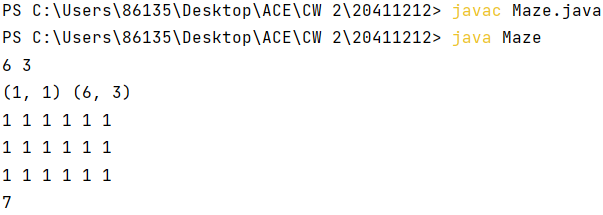
\includegraphics[scale=0.6]{Maze.png}
\caption{Maze}
\end{figure}
Time complexity:\\
The input parsing has a time complexity of $O(n + m)$, where $n$ is the length of the first input line and $m$ is the length of the second input line. The dominant factor is the time complexity of Dijkstra's algorithm: $O(V^2)$ where $V = m * n$.\\
The overall time complexity is $O(n + m + (m*n)^2)$.\\~\\
Space complexity:\\
The maze is represented as a 2D array `maze', contributing $O(m * n)$ to the space complexity. The space complexity related to Dijkstra's algorithm is dominated by the 2D distance array `dist', which is $O(m * n)$, where $m$ is the number of rows and $n$ is the number of columns.\\
The overall space complexity is $O(m * n)$.
\section{Walk}
This java program is about finding the minimal number of steps taken from the start cell to the end cell in an area using DFS (depth-first search) and backtrack.
\subsection{Selection of data structures}
\begin{itemize}
\item ArrayList$<$ArrayList$<$Integer$>>$: Used to represent a 2D ArrayList of integers, e.g.: `all'. It can record all possible routes.
\item int[ ][ ] array: Used to represent a two-dimensional array for the grid where each cell can be either 0 or 1.
\item ArrayList$<$Integer$>$: Use `step' to record the steps in the current path during the DFS process.
\item List$<$Integer$>$: Used to store integers obtained from user input and parsing.
\end{itemize}
\subsection{Algorithm design}
The program is designed to scan and check the area of $n*m$ grid, non-negative int k, the start cell and the end cell from users' input, and use DFS to get and output the minimum number of step it takes from start cell to end cell.\\
\begin{itemize}
\item Read and check input values: Read users' input for grid dimensions ($n$ and $m$), starting and ending coordinates ($(s1, s2)$ and $(e1, e2)$), the number of block cells that can be ignored ($k$), and the grid itself. Then check if the format is right using `isLegal', `isLegalTwoPairs', `isNonNegaInt', `isLegalGrid'.
\item DFS: Define a recursive DFS function `dfsFindWay' to explore possible paths from the starting point to the destination. The DFS function considers different directions: up, down, left, right, upper and lower diagonals, and ignores block cells up to the specified limit `k'. The current path `step' is updated during the DFS traversal.
\item Backtrack: When the destination is reached, record the current path in the all ArrayList, and then backtrack to explore other paths.
\item Find minimun steps and output: After exploring all paths, find the path with the minimum number of steps by iterating through the recorded paths in the `all' ArrayList, then print it out.
\end{itemize}
\subsection{Algorithm correctness justification and efficiency analysis}
The algorithm can run correctly after several different tests, as it successfully output the shortest number of jumping steps.
\begin{figure}[H]
\centering
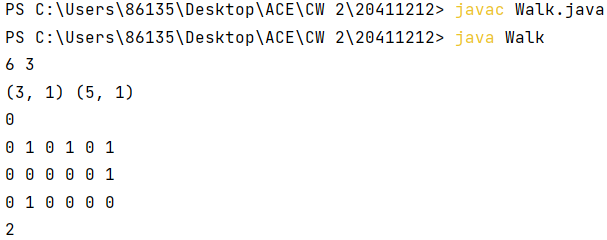
\includegraphics[scale=0.6]{Walk.png}
\caption{Walk}
\end{figure}
Time complexity:\\
Grid validation includes iterating over the input grid and coordinates. Since the grid size and coordinates are bounded by n and m, the complexity of grid validation is $O(n * m)$. The DFS search explores different paths in the grid. In the worst case, it might explore all possible paths, leading to a time complexity of$O(3^{n*m})$, where $3$ represents the number of directions (up, down, left, right, diagonals) excluding the one that led to the current cell.\\
The dominant factor of the overall time complexity is the DFS search, so the overall time complexity is $O(3^{n*m})$.\\~\\
Space complexity:\\
The grid is stored as a 2D array, contributing $O(n * m)$ to the space complexity.\\
The ArrayList `all' stores all recorded paths, and each path is an ArrayList storing coordinates. The space complexity for recorded paths is $O(k * avg)$, where avg is the average length of the recorded paths.
The overall space complexity is $O(n * m + k * avg).$


\end{document}
